\documentclass[11pt]{aghdpl}
% \documentclass[en,11pt]{aghdpl}  % praca w języku angielskim
\usepackage[polish]{babel}
%\usepackage[english]{babel}
\usepackage[utf8]{inputenc}

% dodatkowe pakiety
\usepackage{enumerate}
\usepackage{listings}
\usepackage{graphicx} 
\usepackage{float}
\lstloadlanguages{TeX}

\lstset{
  literate={ą}{{\k{a}}}1
           {ć}{{\'c}}1
           {ę}{{\k{e}}}1
           {ó}{{\'o}}1
           {ń}{{\'n}}1
           {ł}{{\l{}}}1
           {ś}{{\'s}}1
           {ź}{{\'z}}1
           {ż}{{\.z}}1
           {Ą}{{\k{A}}}1
           {Ć}{{\'C}}1
           {Ę}{{\k{E}}}1
           {Ó}{{\'O}}1
           {Ń}{{\'N}}1
           {Ł}{{\L{}}}1
           {Ś}{{\'S}}1
           {Ź}{{\'Z}}1
           {Ż}{{\.Z}}1
}

%---------------------------------------------------------------------------

\author{Mateusz Gruszka}
\shortauthor{M. Gruszka}

\titlePL{Skuteczność algorytmu roju cząstek w wybranych problemach optymalizacji ciągłej}
\titleEN{Effectiveness of particle swarm algorithm in selected continuous optimization problems}

\shorttitlePL{Skuteczność algorytmu roju cząstek w wybranych problemach optymalizacji ciągłej} 
\shorttitleEN{Effectiveness of particle swarm algorithm in selected continuous optimization problems}

\thesistype{Praca dyplomowa magisterska}

\supervisor{dr hab. inż. Marek Kisiel-Dorohinicki}

\degreeprogramme{Informatyka}

\date{2015}

\department{Katedra Informatyki}

\faculty{Wydział Informatyki, Elektroniki i Telekomunikacji}

\acknowledgements{Serdecznie dziękuję \dots tu ciąg dalszych podziękowań które zostaną uzupełnione pod koniec :)}


\setlength{\cftsecnumwidth}{10mm}

%---------------------------------------------------------------------------
\setcounter{secnumdepth}{4}


\begin{document}

\titlepages
\setcounter{tocdepth}{3}
\tableofcontents
\listoffigures

\makeatletter\@openrightfalse

\chapter{Wprowadzenie}
\label{cha:wstep}

Tematem niniejszej pracy jest sprawdzenie skuteczności algorytmu roju cząstek w wybranych problemach optymalizacji ciągłej. Skuteczność rozwiązania została porównana z istniejącym rozwiązaniem zaimplementowanym na platformie pyAgE.

Optymalizacja jest wyznaczeniem spośród dopuszczalnych rozwiązań danego problemu, rozwiązania najlepszego ze względu na przyjęte kryterium (wskaźnik) jakości (np. koszt, zysk, niezawodność). Optymalizacja ciągła jest takim rodzajem optymalizacji, w którym wszystkie zmienne funkcji celu są ciągłe, czyli należą do nieprzerwanego zbioru liczb. Często problemy optymalizacyjne są problemami, w których przestrzeń przeszukiwań jest za duża lub zbyt skomplikowana, żeby można było ją eksplorować jednocześnie wydajnie i dokładnie.

Przy rozwiązywaniu tak złożonych problemów wykorzystywane są heurystyki. Heurystyką nazywamy taką metodę znajdowania rozwiązań, która nie daje gwarancji znalezienia optymalnego rozwiązania. Brak gwarancji znalezienia rozwiązania wynika z faktu, że heurystyki przeszukują przestrzeń rozwiązań i wraz z postępem algorytmu modyfikują jego składowe parametry dostosowywując się do osiąganych wyników pośrednich.

Algorytm roju cząstek, jak również algorytm wykorzystywany w niniejszej pracy w celu porównia skuteczności są heurystykami. Doskonalą one rozwiązanie danego problemu poprzez iteracyjne modyfikowanie parametrów. Algorytmy ewolucyjne czerpią z obserwowanego w przyrodzie procesu ewolucji - podczas działania algorytmu jego najlepiej przystosowane składowe są iteracyjnie modyfikowane, natomiast te przystosowane najgorzej są odrzucane. Algorytm roju cząstek bazuje na zachowaniach stadnych. W każdej kolejnej iteracji elementy algorytmu wpływają na siebie na podstawie swojego położenia w przestrzeni rozwiązań.



\section{Cele pracy}
\label{sec:celePracy}
Celem pracy była implementacja algorytmu roju cząstek oraz zbadanie jego skuteczności w wybranych problemach benchmarkowych. W implementacji zostało wykorzystane istniejące środowisko agentowe - pyAgE. Wspiera ono budowę rozproszonych modeli obliczeniowych oraz dostarcza zestaw narzędzi umożliwiających porównanie zaimplementowanych rozwiązań.

Finalnym celem było porównanie otrzymanych rozwiązań z istniejącym algorytmem ewolucyjnym - EMAS. Aby wykonać porównanie zostały przeprowadzone analizy składowych parametrów wykonanych modyfikacji algorytmu rojowego, a następnie zostały wykorzystane te, które dawały najdokładniejsze rozwiązanie.


\section{Zakres pracy}
W czasie realizacji pracy, zostały stworzone komponenty na platformę pyAgE dające możliwość dokonywania obliczeń za pomocą algorytmu roju cząstek. Zostały zaimplementowane zarówno elementy składowe algorytmu, jak i przetestowane konfiguracje pozwalające na badanie jego skuteczności. 

Porównanie odbywało się na platformie pyAgE pomiędzy istniejącym algorytmem ewolucyjnym EMAS, a różnymi konfiguracjami algorytmu roju cząstek. 

Algorytm roju cząstek został przystosowany, aby sprawdzić jego skuteczność w kilku wersjach:
\begin{itemize}
\item Podstawowa wersja, zawierająca możliwość sterowania:
\begin{itemize}
\item Prędkością
\item Wagami składowych
\end{itemize}
\item Rozszerzoną o kroki algorytmu ewolucyjnego wykonywane razem z rojowymi
\item Rozszerzoną o informację o sąsiadach, dostarczaną przez platformę pyAgE
\item Rozszerzoną o wyspy obliczeniowe
\end{itemize}


\section{Zawartość pracy}
Rozdział \ref{cha:pyage} zawiera informacje o platformie pyAgE i jej komponentach. Znajdują się w nim również informacje o funkcji benchamrkowej stosowanej do porównania wyników niniejszej pracy.

Następną częscią pracy (rozdziały \ref{cha:pso} i \ref{cha:genetyczne}) jest przybliżenie mechanizmów działania zarówno algorytmów rojowych, jak i ewolucyjnych - szczególnie tych, które zostały zastosowane w implementacji. W rodziale \ref{sec:psoModyfikacje} zostały opisane częste modyfikacje algorytmu roju cząstek.

Rozdział \ref{cha:ewaluacja} opisuje sposób zbierania i porównywania otrzymanych wyników. W rozdziale \ref{cha:psoTesty} znajdują się informacje o zaimplementowanych rozwiązaniach oraz wyniki badań prowadzące do uzyskania najlepszych parametrów algorytmu roju cząstek.

Zakończenie pracy poświęcone zostało porównaniu algorytmów rojowego i ewolucyjnego oraz analiza skuteczności algorytmu rojowego pod kątem postawionego problemu.












\chapter{Wieloagentowy system pyAgE}
\label{cha:pyage}
W roku 1997 została zaproponowana definicja agenta, która definiuje go jako ,,system, który usytuowany jest w pewnym środowisku, i którego jednocześnie jest częścią; agent obserwuje (odbiera, odczuwa) to środowisko oraz działa w nim: w czasie, według własnego planu, wpływając na to, co będzie mógł zaobserwować w przyszłości'' \cite{opisagenta}. Definicja powstała na skutek wnikliwej analizy różnych podejść agentowości.

Zgodnie z powyższą definicją, za najistotniejsze cechy agenta należy uznać \cite{agentowyemas}:
\begin{itemize}
\item usytuowanie - agent jest częścią środowiska, w którym się znajduje
\item autonomia - agent ma pełną kontrolę nad swoim stanem wewnętrznym oraz akcjami
\item reaktywność - agent postrzega środowisko i zmiany zachodzące w nim i reaguje na nie
\item zdolności socjalne - agent współdziała z innymi agentami
\end{itemize}

System agentowy to system komputerowy, którego główną abstrakcją jest pojęcie agenta \cite{systemagentowy}. System składający się z wielu współdziałających agentów nazywany jest systemem wieloagentowym. Interakcje między agentami, mogące przyjąć formę kooperacji, koordynacji bądź negocjacji są najistotniejszą cechą charakterystyczną tej klasy systemów i stanowią o ich sile. 

\section{Platforma pyAgE}
\label{sec:pyageopis}
Platformą, na której zostały uruchomione porównywane algorytmy był napisany w języku Python pyAgE \cite{pyagestrona} \cite{pyage}. Jest to środowisko wieloagentowe, bazujące na implementacji pod nazwą AgE (ang. Agent-based Evolution). Platforma AgE powstała na podstawe założeń i wymagań przedstawionych powyżej.

Najważniejszą częścią systemu jest dostarczenie mechanizmu wykonywania obliczeń. Podstawowe elementy implementacji systemu stanowią bazę dla realizacji różnej klasy rozwiązań. Ponadto, dzięki odpowiedniej konfiguracji rozwiązania mogą zostać uruchomione jako sieciowa usługa obliczeniowa.

Jak zostało wspomniane wcześniej, podstawową jednostką składową jest agent, gdzie każdy agent jest unikalny w skali całego systemu. W środowisku można wyróżnić również agregaty, które mogą ,,posiadać'' agentów, którzy współdziałają ze sobą. Agregaty zarządzają działaniem podległych im agentów, między innymi pośredniczą w komunikacji między nimi, nadzorują cykl ich życia czy wykonywanie akcji.

W środowisku dostępne są następujące funkcjonalności:
\begin{itemize}
\item zlecenie przez agenta wykonania pewnej akcji
\item zapytanie przez agenta o własności innych agentów
\item dodanie nowego agenta
\item migracja agenta
\item śmierć agenta
\end{itemize}

Platforma została stworzona z myślą o algorytmach ewolucyjnych, między innymi algorytmie EMAS. Dzięki temu dostarcza mechanizmu wysp obliczeniowych, które są jedną ze składowych części algorytmu EMAS, szerzej opisanego w rozdziale \ref{sec:emas}. To właśnie pomiędzy tymi wyspami możliwa jest migracja poszczególnych agentów.

\section{Rozwinięcie platformy pyAgE}

Jednym z celów pracy było wykonanie implementacji pozwalającej na wykonywanie obliczeń za pomocą algorytmów rojowych. W tym celu zostały wykonane komponenty działające na dostarczonej platformie umożliwiające wykorzystanie takiej klasy algorytmów. 

W analizowanym podejściu każda cząsteczka jest zastępowana przez pojedynczego agenta. Wymagało to rozszerzenia wiedzy agenta o informacje wymagane przez algorytmy rojowe, takie jak najlepsza pozycja w stadzie czy historycznie najlepsza pozycja. Skutkowało to dodaniem dla każdego agenta struktur przechowujących pewne informacje.

Kolejnym etapem było dodanie konfiguracji uruchomieniowej, uwzględniającej możliwość modyfikacji wszystkich istotnych parametrów. Konfiguracja ta, bazująca na już istniejących, nadała możliwość łatwego i szybkiego porównywania dobieranych parametrów, ale także analizy rozwiązań względem istniejących algorytmów.

\chapter{Algorytmy rojowe}
\label{cha:pso}
Algorytmy rojowe, w tym algorytm roju cząstek, należą do algorytmów wykorzystujących inteligencję stadną. Nazywane tak są techniki sztucznej inteligencji bazujące na wiedzy o społecznych zachowaniach w samozorganizowanym systemie \cite{psowstep}. 

Systemy rojowe są najczęściej zbudowane z populacji prostych osobników oddziałujących na siebie nawzajem oraz na środowisko w którym się znajdują. Członkowie populacji nie wykonują skomplikowanych obliczeń, ich wiedza o problemie jest znikoma oraz nie przechowują prawie żadnych informaji. Ponadto nie istnieje scentralizowana struktura kierująca zachowaniem indywidualnych osobników. Jednostki posiadają jedynie wiedzę o akcji jaką powinny podjąć przy danych bodźcach zewnętrznych. Wzajemne oddziaływanie pomiędzy osobnikami prowadzi do złożonych zachowań populacji.

Przykłady takich zachowań są bardzo liczne w naturze. Zaliczyć do nich można kolonie mrówek, klucze ptaków, ławice ryb czy roje pszczół. W przypadkach tych mamy doczynienia z licznymi osobnikami, które wpływając na siebie nawzajem osiągają złożone populacje zdolne realizować skomplikowane zadania.

Algorytmy rojowe dają możliwość szybkiego rozwiązania, jednak ponieważ należą do heurystyk, znalezienie rozwiązania nie jest gwarantowane. Poprzez wykorzystywanie osobników nieposiadających wiedzy o problemie, można wykorzystywać je do rozwiązywania różnych zadań, modyfikując jedynie informację o problemie, jego przestrzeni rozwiązań i funkcji dopasowania. 

\section{Przegląd wiedzy}
\label{sec:historiarojowych}
Pierwszy raz idea wykorzystania zachowań zaobserwowanych w naturze została zaproponowana w 1987 roku \cite{Reynolds87}. Dzięki wykorzystaniu kilku względnie prostych reguł udało się osiągnąć w animacjach symulowanie bardziej skomplikowanych, realistycznie wyglądających zachowań stada ptaków. 

Pojęcie inteligencji stadnej zostało po raz pierwszy użyte w 1989 roku \cite{BeniWang89} w kontekście zrobotyzowanych systemów komórkowych, natomiast w roku 1995 \cite{KennedyEberhart95} pojawiła się pierwsza wersja algorytmu roju cząstek (ang. Particle Swarm Optimization (PSO)). Pierwotnym założeniem algorytmu PSO była symulacja społeczeństwa, jednak problem okazał się zbyt złożony dla takiego algorytmu. Odnalazł on jednak zastosowanie w problemach optymalizacji ciągłej.

Wraz ze wzrostem zainteresowania algorytmami rojowymi, pojawiło się wiele badań i publikacji nad różnymi algorytmami. Do najpopularniejszych i najdokładniej opisanych należy zaliczyć takie jak algorytm mrówkowy (ang. Ant colony optimization (ACO)) \cite{ACO} czy algorytmy pszczele (ang. Bees algorithm (BA)) \cite{BA} i pszczelej kolonii (ang. Artifical bee colony algorithm (ABC)) \cite{ABC}. Część z algorytmów, mimo że ich pierwotne wersje były dostosowane do rozwiązywania problemów dyskretnych, z czasem zostały zmodyfikowane również do rozwiązywania problemów ciągłych. Przykładem takiego algorytmu może być algorytm kolonii mrówek, którego dostosowanie zostało opublikowane ponad dziesięć lat od zaproponowania pierwotnej wersji \cite{ACO2}. 

Ze względu na różnorodność otaczającej przyrody kolejne algorytmy inspirowane naturą są nieustannie proponowane i rozwijane. W momencie pisania niniejszej pracy (rok 2015), jednym z nowszych zaproponowanych jest algorytm lwich mrówek (ang. Ant lion optimizer (ALO)) \cite{ALO}, którego działanie oparte jest na mechanizmach polowania lwich mrówek.

\section{Algorytm roju cząstek}
\label{sec:psoOpis}
Algorytm roju cząstek naśladuje zachowania stadne. Podczas zdobywania doświadczenia (wiedzy), cząsteczki wzajemnie na siebie oddziałują, jednocześnie przesuwając się w coraz lepszy obszar przestrzeni rozwiązań. 

Optymalizacja nie jest wymagająca pod względem zasobów. Zapotrzebowanie na pamięć i czas procesora w każdej iteracji są niskie, a sama zmiana parametrów cząstki odbywa się przy wykorzystaniu podstawowych operatorów matematycznych. Algorytm roju cząstek jest wystarczający dla wielu problemów i nie wymaga skomplikowanych metod używanych na przykład przez algorytmy ewolucyjne.

Każdy osobnik w populacji posiada zestaw mechanizmów warunkujących jego ruch w przestrzeni rozwiązań. Ponadto ma pamięć o najlepszym miejscu w przestrzeni jakie odwiedził oraz wiedzę o położeniu jednostki z najlepszym rozwiązaniem z populacji.

\subsection{Opis algorytmu}
\label{sec:psoRownania}
Jeśli przestrzeń poszukiwań jest D-wymiarowa, można zaprezentować i-tą cząsteczkę populacji jako D-wymiarowy wektor \ref{equ:psoRownanieCzasteczki},

\begin{equation}
\label{equ:psoRownanieCzasteczki}
x_i = (x_{i1}, x_{i2}, x_{i3}, \dots, x_{iD})^T
\end{equation}

gdzie T oznacza numer iteracji. Najlepszą odwiedzoną pozycję (particle best) i-tej cząsteczteczki można oznaczyć jako \ref{equ:psoRownanieNajlepszej}.

\begin{equation}
\label{equ:psoRownanieNajlepszej}
p_{b_i} = (p_{b_{i1}}, p_{b_{i2}}, p_{b_{i3}}, \dots, p_{b_{iD}})
\end{equation}

Na podobnej zasadzie, wprowadzając oznaczenie $g_b$ (global best), oznaczona zostaje najlepsza pozycja w przestrzeni rozwiązań w stadzie. Przyjmując takie oznaczenia, każdy osobnik populacji przemieszcza się według równania ruchu \ref{equ:psoRownanieRuchu}.

\begin{equation}
\label{equ:psoRownanieRuchu}
v_{id}^{n+1} = v_{id}^{n} + (p_{b_{id}}^n - x_{id}^n) + (g_{b_{id}}^n - x_{id}^n)
\end{equation}

co skutkuje, że w kolejnych iteracjach jego pozycja jest uaktualniana zgodnie z równaniem \ref{equ:psoNowaPozycja}
\begin{equation}
\label{equ:psoNowaPozycja}
x_{id}^{n+1} = x_{id}^n + v_{id}^{n+1}
\end{equation}

gdzie:

d = 1, 2, 3, \dots, D

i = 1, 2, 3, \dots, N

N - rozmiar populacji

n = 1,2,3, \dots - numer iteracji

Zgodnie z równaniem \ref{equ:psoRownanieRuchu}, każda nowa pozycja w przestrzeni rozwiązań zależy wyłącznie od poprzednich wartości cząsteczki oraz wartości jej sąsiadów. W celu manipulowania prędkością przesunięcia w konkretnej iteracji, równanie ruchu cząsteczki zostało rozszerzone o współczynnik inercji $\omega$ (\ref{equ:psoFinal}).

\begin{equation}
\label{equ:psoFinal}
v_{id}^{n+1} = \omega(v_{id}^{n} + (p_{b_{id}}^n - x_{id}^n) + (g_{b_{id}}^n - x_{id}^n))
\end{equation}


\subsection{Przemieszczenie}
\label{sec:psoPrzemieszczenie}
Wizualizację zgodnie z równaniami zamieszczonymi w rozdziale \ref{sec:psoRownania}, można prześledzić na rysunku \ref{fig:psoWizualizacja}.

\begin{figure}[H]
\begin{center} 
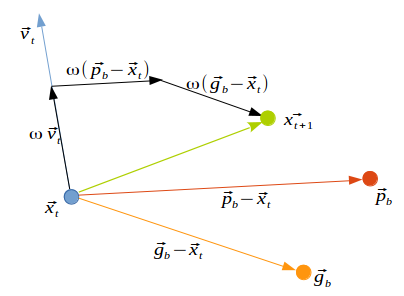
\includegraphics[scale=0.8]{tresc/pics/psoRuch.png}
\caption{Wizualizacja ruchu cząstki PSO}
\label{fig:psoWizualizacja}
\end{center}
\end{figure}

W danej iteracji, cząsteczka znajduje się w konkretnym punkcie $x_t$, zna położenie najlepszej cząsteczki z całej populacji $g_b$ oraz pamięta swoją najlepszą odwiedzoną do tej pory pozycję $p_b$. Osobnik wyzacza wektory przesunięcia względem tych punktów oraz przemieszczenia z poprzedniej iteracji $v_t$. Każdy z wektorów jest mnożony przez współczynnik inercji $\omega$, a następnie wszystkie wektory są ze sobą składane. Wynikiem złożenia jest nowa pozycja cząsteczki w przestrzeni rozwiązań.

\subsection{Zasada działania algorytmu}
\label{sec:psoDzialanie}
Diagram \ref{fig:psoDiagram} przedstawia pełny mechanizm działania algorytmu. Pierwszym krokiem jest zainicjalizowanie startowej populacji w losowych miejscach przestrzeni rozwiązań. Następnie dla każdego osobnika liczone jest dopasowanie, czyli jakość jego rozwiązania. Jeśli aktualne dopasowanie jest lepsze niż zapamiętane, uaktualniana jest pamiętana pozycja w przestrzeni rozwiązań. W przypadku, gdy dopasowanie jest gorsze, zapamiętana informacja pozostaje bez zmian. Kolejnym krokiem jest uaktualnienie informacji najlepszej pozycji z całej populacji. Posiadając wszystkie informacje, cząsteczka wyznacza swoją prędkość w danej iteracji, a następnie przemieszcza się zgodnie z nią w przestrzeni rozwiązań. Aż do spełnienia warunku stopu (uzyskanie pożądanego dopasowania lub osiągnięcia limitu iteracji), cząsteczki ponownie wyliczają swoje dopasowanie i powtarzają cały cykl.

\clearpage

\begin{figure}[H]
\begin{center} 
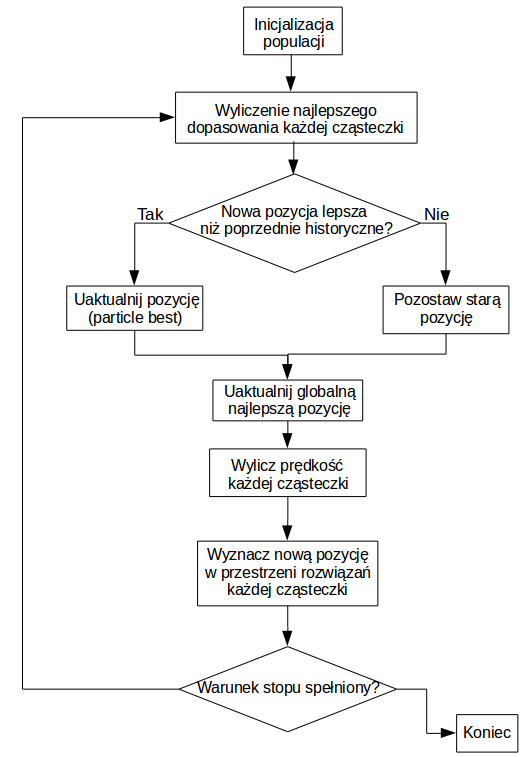
\includegraphics[scale=0.55]{tresc/pics/psoDiagram.png}
\caption{Diagram blokowy algorytmu PSO}
\label{fig:psoDiagram}
\end{center}
\end{figure}


\section{Modyfikacje algorytmu roju cząstek}
\label{sec:psoModyfikacje}
W paragrafie \ref{sec:psoOpis} została przedstawiona podstawowa, najprostsza wersja algorytmu roju cząstek. Istnieje szereg rozszerzeń i modyfikacji algorytmu, które powodują zwiększenie jego dokładności i skuteczności.



\subsection{Rozszerzenie wiedzy cząstek}
\label{sec:psoSasiedztwo}
Rozszerzając wiedzę jednostek o dodatkowe informacje o otoczeniu, często okazuje się, że zwiększa się dokładność, jak i prędkość w jakiej otrzymywany jest satysfakcjonujący wynik. Jednym ze sposobów, jest dodanie wiedzy o położeniu najlepszej cząsteczki w pewnym otoczeniu danego osobnika \cite{PSOneighbourhood}. Dołożenie takiego parametru pociąga za sobą zmianę wyliczania ruchu cząstki (rys. \ref{fig:psoWizualizacja}) o dodatkowy wektor. Podejście takie zwiększa skupienie cząsteczek i pozwala na dokładniejsze przeszukiwanie przestrzeni rozwiązań w danym zakresie. 


\subsection{Dodanie losowej składowej}
\label{sec:psoLosowa}
Uwzględnienie podczas ruchu cząstki dodatkowego składowego wektora, którego wartość oraz kierunek generowane są losowo, daje możliwość pozbycia się pewnych potencjalnych problemów \cite{PSOrandom}. Cząstki które poruszają się w sposób opisany w rozdziale \ref{sec:psoPrzemieszczenie} oraz te rozszerzone o informacje o sąsiedztwie obarczone są ryzykiem wpadania w lokalne ekstrema. Dodając losową składową, wymuszany jest ruch często oddalający osobnika od roju, co może skutkować wyskoczeniem z lokalnego ekstremum i dalszym przeszukiwaniem przestrzeni rozwiązań w celu znalezienia ekstremum globalnego.


\subsection{Nadawanie wag parametrom}
\label{sec:psoWagi}
Podstawowa wersja algorytmu roju cząstek zakłada jednakową wagę każdego z wektorów podczas wyliczania nowej pozycji cząstki. Modyfikacja wprowadzająca dla każdego wektora parametr definiujący jego wagę pozwala na lepsze dostosowanie algorytmu dla danego problemu \cite{PSOparams}.


\subsection{Zmiana prędkości ruchu}
\label{sec:psoPredkosc}
Algorytm roju cząstek w swojej pierwotnej wersji nie zakładał zmiany prędkości osobników w czasie. Rozszerzenie dające możliwość manipulowania współczynnikiem inercji $\omega$ na przestrzeni kolejnych iteracji pozwala na uniknięcie potencjalnego ,,przeskakiwania'' poprawnego rozwiązania przez członków populacji. Wersja podstawowa niesie za sobą ryzyko, że po pewnej ilości iteracji cząsteczki będą krążyły wokół ekstremum, jednak długość wektora będzie zbyt duża, aby udało się im ,,trafić'' w rozwiązanie. Zmniejszanie współczynnika $\omega$ wraz z kolejnymi iteracjami pozwoli cząstkom dokładniej przeszukać dany zakres, jednocześnie utrzymując szeroki zasięg przeszukiwań na początku działania algorytmu \cite{PSOvelocity}.


\chapter{Algorytmy ewolucyjne}
\label{cha:genetyczne}

Algorytmami ewolucyjnymi nazywne są algoytmy, które w celu przeszukania przestrzeni rozwiązań  wykorzystują mechanizmy zaczerpnięte ze zjawiska ewolucji biologicznej. Jest to ogólna nazwa dla metod takich jak algorytmy genetyczne, strategie ewolucyjne czy neuroewolucje. 

Podobnie jak opisane w rozdziale \ref{cha:pso} algorytmy rojowe, ewolucyjne również zawierają populację agentów wpływających nawzajem na siebie. Populacja agentów generowana jest losowo, wraz z pewnym zestawem cech dla każdego agenta - genotypem. Genotyp jest takim zestawem cech agenta, który umiejscawia go w pewnej przestrzeni rozwiązań, co umożliwia jego ewaluację. Podczas działania algorytmu, agenci poprzez krzyżowanie się, umieranie i rodzenie wpływają na swoje genotypy. 

Na przestrzeni lat zostało zaproponowanych wiele algorytmów bazujących na mechanizmach genetycznych, jednak wszystkie z nich opierały się na tych samych bazowych mechanizmach. Każdy z osobników populacji mógł, zmieniając swój genotyp, przybliżyć całą populację do znalezienia optymalnego rozwiązania postawionego problemu. Większość wpółczesnych rozwiązań stosuje również krzyżowanie się osobników, jako drugą główną składową działania algorytmów tego typu.

\section{Przegląd wiedzy}
\label{sec:historiagenetycznych}
Początki algorytmów ewolucyjnych sięgają lat 50 XX wieku\cite{GA1}, jednak ich idee nie były rozwijane przez wiele lat, głównie ze względu na ograniczenia sprzętowe jak i metodologiczne. Dopiero dwadzieścia lat później\cite{GA2} pojawiły się prace rozwijające modele ewolucyjne. Wtedy też zostało zaproponowane twierdzenie Hollanda o schematach, które uważane jest za podstawę wyjaśnienia algorytmów genetycznych. 

Znaczącą kwestią wpływającą na tempo rozwoju algorytmów genetycznych, było użycie techniki uwzględniającej ewolucję zarówno przez mutację jak i krzyżowanie się osobników z danej populacji. Podczas kolejnych lat badań, algorytmy tego typu zostały poszerzone o kod genetyczny pozwalający reprezentować strukturę każdego problemu.

Klasyczne algorytmy ewolucyjne działają zgodnie z algorytmem przedstawionym na diagramie \ref{fig:GAdiagram}, lub podobnie do niego. 

\begin{figure}[H]
\begin{center} 
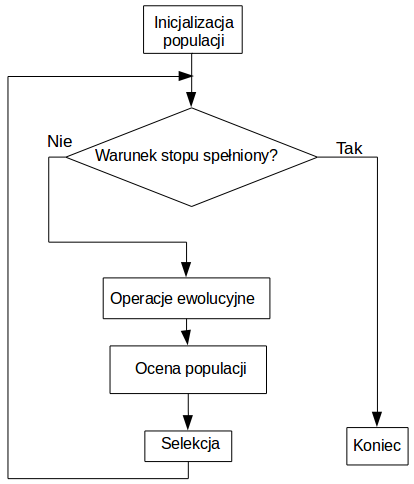
\includegraphics[scale=0.6]{tresc/pics/GAdiagram.png}
\caption{Diagram blokowy klasycznego algorytmu genetycznego}
\label{fig:GAdiagram}
\end{center}
\end{figure}

Początkowo inicjalizowana jest losowa populacja, która wykonuje między sobą zachowania ewolucyjne aż do spełnienia warunku stopu. Podczas każdej iteracji z całej populacji wybierana jest część osobników która zostanie poddana krzyżowaniu się między sobą. Następnie te osobniki poddawane są mutacji. Dla każdego z osobników wyliczana jest funkcja przystosowania, pozwalająca ocenić jakość jego genotypu.

\section{Algorytm EMAS}

Algorytm EMAS (ang. Evolutionary Multi-Agent System) jest paradygmatem obliczeniowym zaproponowanym w 1996 roku\cite{emas1}. Jest to połączenie algorytmu ewolucyjnego z systemem wieloagentowym. Idea algorytmu opiera się na koncepcji, że agenci w środowisku mogą się łączyć, reprodukować i umierać. 

Przeznaczony jest do pracy bez zachowania jakiejkolwiek globalnej wiedzy o problemie. Agenci są niezależni oraz zdolni do podejmowania własnych decyzji dotyczących ich akcji. Ta cecha sprawia, że algorytm jest łatwo skalowalny i pozwala na zrównoleglenie. 

Dziedziczenie i selekcja to dwa główne elementy algorytmów ewolucyjnych, które w algorytmie EMAS realizowane są za pomocą zjawisk śmierci i reprodukcji. Agenci o najlepszym przystosowaniu są zachowane i mogę produkować swoje potomstwo. Agenci o najgorszych parametrach są całkowicie usuwane z otoczenia. Takie zachowanie zmusza populację do ewolucji oraz poprawia jej parametry\cite{emas2}.

\subsection{Agent}
\label{sec:agentgenetyczny}
Każdy z agentów charakteryzuje się trzema parametrami:
\begin {itemize}
\item genotyp (ang. genotype)
\item dopasowanie (ang. fitness)
\item energia (ang. energy)
\end {itemize}
Genotyp agenta stanowi pojedynczą odpowiedź na zadany problem populacji. Jest to podstawa do obliczenia dopasowania. Genotyp jest cechą dziedziczoną podczas reprodukcji i ulega mutacji w procesie ewolucji. Jako zasadniczy parametr agenta jest to podstawa dla pozostałych parametrów.

Kolejną cechą jest dopasowanie, które jest liczbą reprezentującą jakość genotypu. Lepsze genotypy mają lepsze wartości dopasowania i mają większe prawdopodobieństwo aby być wybranym przy procesie reprodukcji. Sama wartość jest obliczana bezpośrednio z parametru genotypu po stworzeniu agenta. Dopasowanie danego agenta, tak samo jak jego genotyp nie zmienia sie w czasie jego życia.

Ostatnią cechą, wpływającą na sposób selekcji jest energia. Ze względu na brak globalnej wiedzy agentów, nie jest możliwa ocena ich wszystkich w tym samym czasie. Ponieważ proces ewolucji jest asynchroniczny, metody selekcji znane z klasycznych algorytmów ewolucyjnych nie mogły zostać użyte. Z tego powodu została wprowadzona energia, można opisać ten parametr jako stan agenta, który podczas interakcji może ją zyskiwać lub tracić, zależnie od jakości genotypu. Agenci z lepszym genotypem są bardziej skłonni do gromadzenia energii, jednak całkowita ilość energii w populacji jest stała.

Ponieważ agenci w algorytmie EMAS są całkowicie autonomiczni, decyzję o swoim zachowaniu podejmują na podstawie poziomu energii. Jeśli jej liczba przekracza pewien próg to będą się reprodukować, a jeśli osiągnie zero to agent umiera\cite{emas3}.


\subsection{Interakcje agentów}
Istnieją trzy możliwe działania agenta, które może podjąć w danym kroku iteracji:
\begin{itemize} 
\item śmierć (ang. death) 
\item reprodukcja (ang. reproduction) 
\item walka (ang. fight) 
\end{itemize}

Śmierć to usunięcie agenta z populacji, spowodowane jest najczęściej poprzez osiągnięcie przez danego agenta zerowego poziomu energii.

Reprodukcja jest procesem tworzenia nowych agentów. Wymaga wystąpienia jednego lub dwójki rodziców i skutkuje odpowiednio jednym lub dwójką nowo powstałych agentów. Jak zostało wspomniane w rozdziale \ref{sec:agentgenetyczny}, rozwiązanie oraz dopasowanie są stałe podczas życia agenta, więc ich wartość u rodziców się nie zmienia. Jedyną zmianą parametru jest zmniejszenie ich poziomu energii, która jest przekazywana nowopowstałym agentom. Genotypy nowo narodzonych agentów są tworzone poprzez losowe zmieszanie genotypów ich rodziców. W momencie uzyskania genotypu, możliwe jest obliczenie dopasowania danego agenta.

Walka jest działaniem odpowiedzialnym za wymianę energii. Dzięki niej, agenci o lepszym genotypie są w stanie pobrać energię od tych z gorszym. Walka sprowadza się do porównaniu dopasowania dwóch agentów i w jego efekcie transferze energii. Jest to szybki sposób porównania i nagradzania najlepszych rozwiązań.

Jak zostało wspomniane wcześniej, ilość energii jest stała w całym układzie. W wyniku reprodukcji nowo narodzony agent dostaje energię od rodziców, natomiast w przypadku walki następuje wymiana pomiędzy dwoma agentami.

\subsection{Ewolucja}

Pomimo, że proces ewolucji jest asynchorniczny można zauważyć pewien schemat zachowania, przedstawiony na rysunku \ref{fig:emasdiagram}.

\begin{figure}[H]
\begin{center} 
\includegraphics[scale=0.6]{tresc/pics/emasdiagram.png}
\caption{Operacje ewolucyjne w algorytmie EMAS}
\label{fig:emasdiagram}
\end{center}
\end{figure}

Pierwszym krokiem jest zdecydowanie jakie działania powinien podjąć agent w danej iteracji. Ponieważ nie ma żadnej wiedzy globalnej, jego decyzje opierają się wyłącznie o jego parametry. Wszyscy agenci zostają oznaczeni jaką akcję podejmą w danym kroku.

Następnie agenci są dzieleni na trzy grupy, odpowiednio dla akcji które zostaną podjęte. Ma to na celu spowodowanie współdziałania ich ze sobą. Ponieważ agenci nie wiedzą jakie działania podejmą pozostali, ten krok jest wymagany aby spowodować interakcje wewnątrz populacji.

Kolejnym krokiem jest przeprowadzenie akcji wewnątrz grup. Część agentów umiera, a część powstaje, zależnie od składu grup. W ostatnim kroku agenci są zbierani w całość, a następnie przemieszani. Ma to na celu uniknięcie ciągłej interakcji ze sobą tych samych agentów.


\subsection{Wyspy obliczeniowe}
Populacją nazywany jest cały zbiór agentów, Jej początkowy rozmiar jest parametryzowany i zmienia się w czasie wykonywania programu. Interakcje wewnątrz populacji nie odbiegają zbytnio od większości algorytmów ewolucyjnych.

Podczas pojedynczego przebiegu programu można utworzyć wiele różnych populacji nazywanych wyspami\cite{emas3}, zmieniających się niezależnie w tym samym czasie. 

Poprzez wprowadzenie migracji między różnymi wyspami, jest możliwe eksportowanie pewnych rozwiązań pomiędzy wyspami, co ma pozytywny wpływ na ogólną wydajność. Dobre rozwiązanie opracowane w jednej populacji może być wprowadzone do innej, powodując modyfikację genotypu. 

Wprowadzenie wysp obliczeniowych dodaje każdemu agentowi dodatkową akcję jaką może podjąć, a mianowicie migrację. Jak wszystkie pozostałe akcje, zależna jest ona od wartości energii danego agenta.




\chapter{Wybrane aspekty realizacyjne}
\label{cha:ewaluacja}

Wszystkie konfiguracje implementacji zostały przetestowane i porównane na podstawie wielowymiarowej funkcji Rastrigina, opisanej w rozdziale \ref{sec:rastrigin} oraz przy wykorzystaniu takiego samego sprzętu. Na sprzęcie był zainstalowany system operacyjny Ubuntu 14.04LTS. Obliczenia były wykonywane na procesorze Intel Core 2 Duo CPU T9600 taktowanym częstotliwością 2.80GHz na każdy z dwóch rdzeni i 8GB pamięci RAM DDR3 taktowanej 1333MHz.

\section{Platforma implementacyjna}
\label{sec:pyageopis}
Platformą, na której zostały uruchomione porównywane algorytmy był napisany w języku Python pyAgE\footnote{https://github.com/maciek123/pyage} \cite{pyage}. Jest to środowisko wieloagentowe, bazujące na implementacji pod nazwą AgE (ang. Agent-based Evolution). Platforma AgE powstała na podstawe założeń i wymagań przedstawionych powyżej.

Najważniejszą częścią systemu jest dostarczenie mechanizmu wykonywania obliczeń. Podstawowe elementy implementacji systemu stanowią bazę dla realizacji różnej klasy rozwiązań. Ponadto, dzięki odpowiedniej konfiguracji rozwiązania mogą zostać uruchomione jako sieciowa usługa obliczeniowa.

Jak zostało wspomniane wcześniej, podstawową jednostką składową jest agent, gdzie każdy agent jest unikalny w skali całego systemu. W środowisku można wyróżnić również agregaty, które mogą ,,posiadać'' agentów, którzy współdziałają ze sobą. Agregaty zarządzają działaniem podległych im agentów, między innymi pośredniczą w komunikacji między nimi, nadzorują cykl ich życia czy wykonywanie akcji.

W środowisku dostępne są następujące funkcjonalności:
\begin{itemize}
\item zlecenie przez agenta wykonania pewnej akcji
\item zapytanie przez agenta o własności innych agentów
\item dodanie nowego agenta
\item migracja agenta
\item śmierć agenta
\end{itemize}

Platforma została stworzona z myślą o algorytmach ewolucyjnych, między innymi algorytmie EMAS. Dzięki temu dostarcza mechanizmu wysp obliczeniowych, które są jedną ze składowych części algorytmu EMAS, szerzej opisanego w rozdziale \ref{sec:emas}. To właśnie pomiędzy tymi wyspami możliwa jest migracja poszczególnych agentów.

\section{Metodyka prowadzenia eksperymentów}
Startowa populacja dla wszystkich konfiguracji wynosiła 360 agentów. Warunkiem stopu dla algorytmów było osiągnięcie globalnego minimum (które dla funkcji Rastrigina wynosi 0) lub przekroczenie limitu 3000 iteracji. Wszystkie eksperymenty zostały powtórzone trzydziestokrotnie, a przedstawiane wyniki zostały uśrednione z zawartym odchyleniem standardowym.

Dla algorytmu EMAS, mutacja była wykonywana poprzez losową modyfikację każdego z genów w genotypie. Krzyżowanie odbywało się poprzez podzielenie genotypów rodziców w jednym miejscu, a potomek otrzymywał po jednej części od każdego z rodziców. Można to zaobserwować na rysunku \ref{fig:spc}. Agenci byli zainicjalizowani z energią równą 100, a pozostałe wartości energii prezentowały się następująco:

\begin{itemize}
\item śmierć agenta = 0
\item minimum dla reprodukcji = 90
\item minimum dla migracji = 120
\item energia dla nowonarodzonych agentów = 100
\item transfer energii = 40
\end{itemize}


\begin{figure}[H]
\begin{center} 
\includegraphics[scale=0.5]{tresc/pics/singlepointcrossover.png}
\caption{Krzyżowanie}
\label{fig:spc}
\end{center}
\end{figure}

\clearpage

\section{Sposób porównywania wyników}
\label{sec:porownywanieWynikow}

W celu porównania jakości algorytmów, podczas obliczeń zbierane były informacje o:
\begin{itemize}
\item Wartości funkcji dopasowania - fitness
\item Różnorodności agentów w populacji:
\begin{itemize}
\item Różnorodność MSD
\item Różnorodność MOI
\end{itemize}
\item Liczebności populacji
\item Czasie obliczeń
\end{itemize}

Wartość funkcji dopasowania jest głównym kryterium oceny jakości danego algorytmu. Na jej podstawie podczas eksperymentów zostały odrzucane pewne rozwiązania, a inne były rozwijane. Jej wartość informuje jak blisko optymalnego rozwiązania znajduje się rozwiązanie wypracowane przez populację. Im wartość funkcji bliższa zeru, tym jakość rozwiązania jest lepsza.

Różnorodność populacji była mierzona za pomocą dwóch kryteriów, MSD oraz MOI, które zostały szczegółowo opisane w rozdziale \ref{sec:roznorodnosc}. Wartość różnorodności informuje jak bardzo genotyp agentów różni się pomiędzy sobą. Większa różnorodność informuje o szerszym przeszukiwaniu przestrzeni rozwiązań przez populację oraz zmniejsza ryzyko utknięcia w lokalnym ekstremum.

Podczas działania algorytmu EMAS liczebność populacji zmienia się w skutek śmierci i rozmnażania agentów. W przypadku algorytmu roju cząstek populacja początkowa nie zmienia swojej liczebności. W rozdziale \ref{cha:psovsemas}, w którym porównywane są algorytmy EMAS i PSO, znajdują się informacje o zmianie liczebności populacji w kolejnych iteracjach.

Dla każdej konfiguracji mierzony był czas obliczeń, który prezentowany jest w formie uśrednionego wyniku.


\section{Problem testowy}
\label{sec:rastrigin}

Funkcja Rastrigina, zaproponowana w 1974 roku \cite{rastrigin}, używana jest jako problem testu wydajności dla algorytmów optymalizacji. Jest to funkcja nieliniowa. Znalezienie minimum funkcji jest stosunkowo trudnym problemem, ze względu na dużą przestrzeń poszukiwań i istnienie wielu minimów lokalnych, co można zaobserwować na rysunku \ref{fig:rastrigin_function} wizualizującym funkcję dla dwóch zmiennych.

\begin{figure}[H]
\begin{center} 
\includegraphics[scale=0.3]{tresc/pics/rastrigin_function.png}
\caption{Funkcja Rastrigina dwóch zmiennych\footnotemark} 
\label{fig:rastrigin_function}
\end{center}
\end{figure}

\footnotetext{http://commons.wikimedia.org/wiki/File:Rastrigin function.png}
Funkcja została zgeneralizowana do n zmiennych w 1991 roku \cite{rastrigin2} i jej ogólną wersję można opisać wzorem \ref{equ:funkcjarastriginawielowymiarowa}. 

\begin{equation}
 f(x) = A n + \sum_{i=1}^n(x_{i}^2 - A cos(2 \pi x_{i}))
 \label{equ:funkcjarastriginawielowymiarowa}
\end{equation}

We wszystkich badaniach porównujących jakość zaimplementowanych rozwiązań używana jest 40-wymiarowa funkcja Rastrigina. Jej parametr $A$ jest równy 10, natomiast wartości przyjmowane przez $x$ należą do przedziału $[-10, 10]$.

\section{Badanie różnorodności populacji}
\label{sec:roznorodnosc}

W celu porównania rozwiązań agentów w populacji zastosowane zostały dwie miary różnorodności: MSD i MOI. Większa różnorodność populacji informuje o szerszym przeszukiwaniu przestrzeni rozwiązań, co pozwala uniknąć utknięcia w lokalnych ekstremach danego problemu.

\subsection*{Różnorodność MSD}
Pierwszym sposobem mierzenia różnorodności jest MSD (ang. maximum standard deviation), czyli maksymalne odchylenie standardowe. 

Maksymalne odchylenie standardowe każdego genu obliczone dla wszystkich agentów w populacji skupia się na dyspersji średnich wartości obliczonych dla poszczególnych genów \cite{roznorodnosckisiel}.

\subsection*{Różnorodność MOI}
Drugim rodzajem różnorodności jest różnorodność MOI (Morrison-De Jong) \cite{roznorodnoscmoi}. W sposobie tym pomiar oparty jest na koncepcji momentu bezwładności dla środka ciężkości populacji. Środek ciężkości obliczany jest dla punktów rozproszonych w wielowymiarowej przestrzeni. Podejście takie pozwala na skuteczny pomiar rozkładu masy w dowolnie wielowymiarowych przestrzeniach. 

Miara opierająca się o inercję została zdefiniowana wzorem \ref{equ:moi}, gdzie $c_j$ to współrzędne środka masy, natomiast $x_{ij}$ oznacza wartość i-tego genu w j-tym chromosomie.

\begin{equation}
 I = \sum_{i=1}^n\sum_{j=1}^N(x_{ij} - c_j)^2
 \label{equ:moi}
\end{equation}



\chapter{Algorytm roju cząstek na platformie PyAGE}
\label{cha:psoTesty}



rozdział o różnych parametrach pso, porównanie wszystkich implementacji, eksperymenty z parametrami itp.

\section{rowne wagi}
\section{stala predkosc}
\section{dodanie losowego wspolczynnika}








\chapter{Porównanie algorytmów genetycznego i PSO}
\label{cha:psovsemas}


tutaj będą te wszystkie wykresy które do tej pory konsultowaliśmy, i wszystkie ich opisy itp.
tutaj juz beda tylko takie pso(pso, pso+sasiedztwo, pso+wyspy) ktore w poprzednim rozdziale bylo jako najlepsze


\section{1 wyspa}
\section{3 wyspy}
\section{6 wysp}
\section{9 wysp}
\section{12 wysp}
\section{porównanie czasu działania}

\chapter{Podsumowanie}
\label{cha:podsumowanie}

W pracy zaproponowano implementację algorytu roju cząstek oraz zbadano jego skuteczność w wybranym problemie benchmarkowym, funkcji Rastrigina. Do platformy pyAgE zostały dodane komponenty umożliwiające dokonanie obliczeń za pomocą algorytmów rojowych, które następnie zostały porównane z EMAS.

Został przeanalizowany szereg konfiguracji i rozszerzeń algorytmu roju cząstek. Szczegółowe wyniki porównujące jakość zaimplementowanego algorytmu pod kątem różnych jego modyfikacji znajdują się w rozdziale \ref{cha:psoTesty}. Spośród sprawdzanych rozwiązań zostało wybrane dające najlepszą wartość dopasowania, a następnie porównane z istniejącą implementacją algorytmu EMAS. Aby w pełni wykorzystać platformę obliczeniową, zostały wykonane modyfikacje algorytmu roju cząstek w oparciu o elementy przez nią dostarczane. W rozdziale \ref{cha:psovsemas} znajduje się porównanie jakości rozwiązań otrzymywanych poprzez wykorzystanie takich modyfikacji.

Wykonane analizy skuteczności algorytmu roju cząstek wykazały, że wykorzystanie wieloagentowej platformy do implementacji algorytmów rojowych daje wyniki mogące konkurować z algorytmami ewolucyjnymi. Jak można zaobserwować na podstawie danych przedstawionych w rozdziale \ref{cha:psovsemas}, algorytm PSO radzi sobie niewiele gorzej niż EMAS. Zdecydowaną zaletą badanego rozwiązania jest liczba iteracji w jakiej algorytm rojowy osiąga stosunkowo zadowalającą wartość funkcji dopasowania. EMAS na osiągnięcie podobnej jakości potrzebuje ponad dwukrotnie większej liczby iteracji.

Przy wykorzystaniu jednej wyspy obliczeniowej już w momencie pięćsetnej iteracji wartość dopasowania dla rozwiązania jest zauważalnie lepsza niż dla algorytmu EMAS, co pozwala na szybkie prototypowanie przy rozwiązywaniu bardziej skomplikowanych problemów. Z drugiej jednak strony, wraz z postępem obliczeń wzrost jakości nie jest już tak szybki.

Wykorzystywanie rozwiązań dostarczonych przez platformę pyAgE, jak również połączenie algorytmów rojowego z ewolucyjnym dało pozytywny skutek. Rozszerzenie wiedzy agenta będącego cząsteczką roju o wiedzę na temat rozwiązania wypracowanego przez jego sąsiadów i dodanie najlepszego z nich jako wektora składowego pozwoliło na skuteczne konkurowanie z rozwiązaniami wypracowywanymi przez EMAS. Wraz z postępem iteracji jakość rozwiązania opracowywana przez rój jest stale poprawiana i przy wykorzystaniu jednej wyspy obliczeniowej jest w stanie konkurować z algorytmem ewolucyjnym.

Wykonywanie przez każdego agenta na początku każdego kolejnego kroku elementów algorytmu ewolucyjnego, a następnie rojowego zgodnie z oczekiwaniami spowodowało wzrost czasu wykonywania, jednak pozwoliło na opracowywanie najlepszych rozwiązań. Połączenie algorytmów pozwala na początkowo szybsze przybliżanie się do globalnego ekstremum niż algorytm EMAS, a wraz z postępem iteracji pozwala na szybsze dalsze udoskonalania iteracji niż algorytm PSO. 



%\section{Możliwy rozwój}
Ponieważ algorytm roju cząstek jest algorytmem umożliwiającym łatwe modyfikacje, możliwe jest wprowadzenie dodatkowych parametrów warunkujących ruch cząstki. Jedną z przykładowych możliwych modyfikacji może być wykorzystanie sąsiedztwa innych cząstek w przestrzeni rozwiązań jako kolejnej składowej. 

Podczas eksperymentów zauważalny był spadek jakości rozwiązań algorymtu rojowego względem ewolucyjnego w przypadku zwiększenia liczby wysp obliczeniowych. Jest to pole do dalszych ulepszeń, które mogą skutkować lepszym wykorzystaniem dostarczanych przez platformę mechanizmów. Umożliwienie migracji cząstek pomiędzy wyspami spowodowałoby zmniejszenie ryzyka utknięcia roju w lokalnym minimum.

Inteligencja stadna jest szeroko rozwijaną koncepcją, o czym świadczyć może długa i ciągle rozszerzająca się lista algorytmów inspirowanych naturą \cite{listaswarm}. Dzięki prostemu interfejsowi dostarczanemu przez platformę, jak i prostym mechanizmom konfigurowania i testowania rozwiązań, możliwe jest szybkie sprawdzanie skuteczności nowych algorytmów stadnych. 







\@openrighttrue\makeatother




% itd.
% \appendix
% \include{dodatekA}
% \include{dodatekB}
% itd.


\bibliographystyle{alpha}
\bibliography{bibliografia}
\begin{thebibliography}{1}

\bibitem{Reynolds87}
C. W. Reynolds
\newblock {\em Flocks, Herds, and Schools: A Distributed Behavioral Model}.
\newblock Computer Graphics, 21(4), Lipiec 1987, str. 25-34

\bibitem{BeniWang89}
G. Beni, J. Wang
\newblock {\em Swarm Intelligence in Cellular Robotic Systems}.
\newblock NATO Advanced Workshop on Robots and Biological Systems, Włochy, Lipiec 1989

\bibitem{KennedyEberhart95}
J. Kennedy, R. Eberhart
\newblock {\em Particle Swarm Optimization}.
\newblock Proceedings of IEEE International Conference on Neural Networks IV, 1995, str. 1942–1948


\bibitem{ABC}
D. Karaboga
\newblock {\em An Idea Based On Honey Bee Swarm for Numerical Optimization}.
\newblock  Technical Report-TR06, Erciyes University, Engineering Faculty, Computer Engineering Department, Turcja, 2005


\bibitem{BA}
D.T. Pham, A. Ghanbarzadeh, E. Koç, S. Otri , S. Rahim , M. Zaidi 
\newblock {\em The Bees Algorithm – A Novel Tool for Complex Optimisation Problems}.
\newblock Technical Note, Manufacturing Engineering Centre, Cardiff University, Wielka Brytania, 2005


\bibitem{ACO2}
X. Hu, J. Zhang, Y. Li
\newblock {\em Orthogonal methods based ant colony search for solving continuous optimization problems}.
\newblock Journal of Computer Science and Technology, Springer, Styczeń 2008, str. 2-28


\bibitem{ACO}
M. Dorigo, L.M. Gambardella
\newblock {\em Ant Colony System : A Cooperative Learning Approach to the Traveling Salesman Problem}.
\newblock IEEE Transactions on Evolutionary Computation, 1997, str. 53-66


\bibitem{ALO}
S. Mirjalili
\newblock {\em The Ant Lion Optimizer}.
\newblock Advances in Engineering Software 83, 2015, str. 80–98.


\bibitem{PSOneighbourhood}
P.N. Suganthan
\newblock {\em Particle swarm optimiser with neighbourhood operator}.
\newblock Evolutionary Computation, IEEE, Washington, 1999


\bibitem{PSOrandom}
M. Clerc
\newblock {\em Standard Particle Swarm Optimisation}.
\newblock HAL open access archive, 2012


\bibitem{PSOparams}
Y. Shi, R.C. Eberhart
\newblock {\em Parameter selection in particle swarm optimization}.
\newblock Evolutionary Computation, IEEE, Washington, 1999
Proceedings of Evolutionary Programming VII (EP98), 1998


\bibitem{PSOvelocity}
R.C. Eberhart, Y. Shi
\newblock {\em Comparing inertia weights and constriction factors in particle swarm optimization}.
\newblock Proceedings of the Congress on Evolutionary Computation 1, 2000


\bibitem{GA1}
G.E.P. Box 
\newblock {\em Evolutionary operation: A method for increasing industrial productivity}.
\newblock Appl. Statistics, vol. VI, no.2, 1957, str. 81–101


\bibitem{GA2}
J. H. Holland
\newblock {\em Adaptation in Natural and Artificial Systems}.
\newblock  University of Michigan Press, Ann Arbor, 1975


\bibitem{EMASweb}
A. Byrski, R. Dreżewski, M. Kisiel-Dorohinicki, L. Siwik
\newblock {\em Evolutionary Multi-Agent Systems}.
\newblock  AGH University of Science and Technology, 2012
\newblock \\\texttt{https://age.iisg.agh.edu.pl/emas/emas.html}.
\newblock Data dostępu: 05.07.2015


\bibitem{emas1}
K. Cetnarowicz, M. Kisiel-Dorohinicki, E. Nawarecki
\newblock {\em The application of evolution process in multi-agent world (MAW) to the prediction system}.
\newblock  M. Tokoro, editor, Proc. of the 2nd Int. Conf. on Multi-Agent Systems (ICMAS'96). AAAI Press, 1996


\bibitem{emas2}
 A. Byrski, R. Drezewski, L. Siwik, M. Kisiel-Dorohinicki
\newblock {\em Evolutionary multiagent systems}.
\newblock The Knowledge Engineering Review, 2013


\bibitem{emas3}
M. Kisiel-Dorohinicki
\newblock {\em Agent-oriented model of simulated evolution}.
\newblock In William I. Grosky and Frantisek Plasil, editors, SofSem 2002: Theory and Practice of Informatics, volume 2540 of LNCS. Springer-Verlag, 2002.


%\bibitem{rastrigin}
%Wikimedia Commons
%\newblock {\em Rastrigin function}.
%\newblock \\\texttt{http://commons.wikimedia.org/wiki/File:Rastrigin function.png}.


\bibitem{agentowyemas}
M. Kisiel-Dorohinicki
\newblock {\em Agentowe architektury populacyjnych systemów inteligencji obliczeniowej}.
\newblock Rozprawy monograficzne 269, Wydawnictwo AGH, Kraków, 2013


\bibitem{opisagenta}
S. Franklin, A. Graesser
\newblock {\em Is it an agent or just a program?: A taxonomy for antonomous agents.}.
\newblock Intelligent Agents III vol. 1193, LNAI. Springer-Verlag, 1997


\bibitem{systemagentowy}
M. Wooldridge
\newblock {\em Agent-based Software Engineering.}.
\newblock IEEE Trans. on Software Engineering, vol. 144, no. 1, 1997


\bibitem{pyage}
M. Kaziród, W. Korczynski, A. Byrski.
\newblock {\em Agent-oriented computing platform in python.}.
\newblock  Web Intelligence (WI) and Intelligent Agent Technologies (IAT), 2014 IEEE/WIC/ACM International Joint Conferences on, vol. 3, pages 365-372. IEEE, 2014


\bibitem{rastrigin}
L. A. Rastrigin
\newblock {\em Systems of extremal control.}.
\newblock Nauka, Moskwa, 1974


\bibitem{rastrigin2}
 H. Mühlenbein, D. Schomisch, J. Born
\newblock {\em The Parallel Genetic Algorithm as Function Optimizer.}.
\newblock Parallel Computing, 17, 1991


\bibitem{roznorodnosckisiel}
M. Kisiel-Dorohinicki
\newblock {\em Evolutionary multi-agent systems in non-stationary environments.}
\newblock Computer Science 14, 2013


\bibitem{roznorodnoscmoi}
R. W. Morrison, K. A. D. Jong 
\newblock {\em Measurement of Population Diversity. In: Artificial Evolution.}
\newblock 5th Int. Conf., Evolution Artificielle, EA 2001, P. Collet, et al., eds., LNCS, vol. 2310, Springer, 2002


\bibitem{listaswarm}
I. Fister, X.S. Yang, J. Brest, D. Fister
\newblock {\em A Brief Review of Nature-Inspired Algorithms for Optimization.}
\newblock Elektrotehniski Vestnik, 80 , 2013

%\bibitem{pyagestrona}
%M. Kaziród
%\newblock {\em pyAgE github}.
%\newblock \\\texttt{https://github.com/maciek123/pyage}.

\bibitem{psowstep}
U. Boryczka
\newblock {\em Inteligencja stadna}.
\newblock \\\texttt{http://155.158.112.34/algorytmyewolucyjne/materialy/inteligencja stadna.pdf}.
\newblock Data dostępu: 05.07.2015


\end{thebibliography}



\end{document}
